\section{Online Aggregation}
\label{sec:online}

Although MapReduce was originally designed as a batch-oriented system,
it is often used for interactive data analysis: a user submits a job
to extract information from a data set, and then waits to view the
results before proceeding with the next step in the data analysis
process. This trend has accelerated with the development of high-level
query languages that are executed as MapReduce jobs, such as
Hive~\cite{hive}, Pig~\cite{pig}, and Sawzall~\cite{sawzall}.

Traditional MapReduce implementations provide a poor interface for interactive
data analysis, because they do not emit any output until the job has been
executed to completion. In many cases, an interactive user would prefer a
``quick and dirty'' approximation over a correct answer that takes much longer
to compute. In the database literature, online aggregation has been proposed to
address this problem~\cite{onlineagg}, but the batch-oriented nature of
traditional MapReduce implementations makes these techniques difficult to
apply. In this section, we show how we extended our pipelined Hadoop
implementation to support online aggregation within a single job
(Section~\ref{sec:online-single}) and between multiple jobs
(Section~\ref{sec:online-multi}). In Section~\ref{sec:online-eval}, we evaluate
online aggregation on two different data sets, and show that it can yield an
accurate approximate answer long before the job has finished executing.

\subsection{Single-Job Online Aggregation}
\label{sec:online-single}

In HOP, the data records produced by map tasks are sent to reduce tasks shortly
after each record is generated. However, to produce the final output of the job,
the reduce function cannot be invoked until the entire output of every map task
has been produced. We can support online aggregation by simply applying the
reduce function to the data that a reduce task has received so far. We call the
output of such an intermediate reduce operation a \emph{snapshot}.

Users would like to know how accurate a snapshot is: that is, how
closely a snapshot resembles the final output of the job. Accuracy
estimation is a hard problem even for simple SQL queries~\cite{dbo}, 
and particularly hard for jobs where the map and reduce
functions are opaque user-defined code. Hence, we report job \emph{progress}, not
accuracy: we leave it to the user (or their MapReduce code) to correlate
progress to a formal notion of accuracy.  We give a simple progress metric below.

Snapshots are computed periodically, as new data arrives at each reducer. The
user specifies how often snapshots should be computed, using the progress metric
as the unit of measure. For example, a user can request that a snapshot be
computed when 25\%, 50\%, and 75\% of the input has been seen. The user may also
specify whether to include data from tentative (unfinished) map tasks. This
option does not affect the fault tolerance design described in
Section~\ref{sec:ft}. In the current prototype, each snapshot is stored in a
directory on HDFS\@. The name of the directory includes the progress value
associated with the snapshot. Each reduce task runs independently, and at a
different rate. Once a reduce task has made sufficient progress, it writes a
snapshot to a temporary directory on HDFS, and then atomically renames it to the
appropriate location.

Applications can consume snapshots by polling HDFS in a predictable
location. An application knows that a given snapshot has been
completed when every reduce task has written a file to the snapshot
directory.  Atomic rename is used to avoid applications mistakenly
reading incomplete snapshot files.

Note that if there are not enough free slots to allow all the reduce tasks in a
job to be scheduled, snapshots will not be available for reduce tasks that are
still waiting to be executed. The user can detect this situation (e.g.,\ by
checking for the expected number of files in the HDFS snapshot directory), so
there is no risk of incorrect data, but the usefulness of online aggregation
will be reduced. In the current prototype, we manually configured the cluster to
avoid this scenario. The system could also be enhanced to avoid this pitfall
entirely by optionally waiting to execute an online aggregation job until there
are enough reduce slots available.

\subsubsection{Progress Metric}
\label{sec:online-metric}
Hadoop provides support for monitoring the progress of task
executions. As each map task executes, it is assigned a \emph{progress
  score} in the range [0,1], based on how much of its input the map
task has consumed. We reused this feature to determine how much
progress is represented by the current input to a reduce task, and
hence to decide when a new snapshot should be taken.

First, we modified the spill file format depicted in
Figure~\ref{fig:mapoutput} to include the map's current progress
score. When a partition in a spill file is sent to a reducer, the
spill file's progress score is also included. To compute the progress
score for a snapshot, we take the average of the progress scores
associated with each spill file used to produce the snapshot.

Note that it is possible that a map task might not have pipelined
\emph{any} output to a reduce task, either because the map task has
not been scheduled yet (there are no free {\TT} slots), the map tasks does 
not produce any output for the given reduce task, or because the reduce task has 
been configured to only pipeline data from at most $k$ map tasks concurrently. 
To account for this, we need to scale the progress metric to reflect the portion 
of the map tasks that a reduce task has pipelined data from: if a reducer is 
connected to $\frac{1}{n}$ of the total number of map tasks in the job, we divide
the average progress score by $n$.

This progress metric could easily be made more sophisticated: for example, an
improved metric might include the selectivity ($|output|/|input|$) of each map task, the
statistical distribution of the map task's output, and the effectiveness of each
map task's combine function, if any. 
% We also assume that each map task
% constitutes a random sample from the input file; otherwise, the scale
% factor we use to account for unavailable map input will introduce
% bias. 
Although we have found our simple progress metric to be
sufficient for most experiments we describe below, this clearly
represents an opportunity for future work.

\subsection{Multi-Job Online Aggregation}
\label{sec:online-multi}

Online aggregation is particularly useful when applied to a long-running
analysis task composed of multiple MapReduce jobs.  As described in
Section~\ref{sec:inter-pipe}, our version of Hadoop allows the output of a
reduce task to be sent directly to map tasks. This feature can be used to
support online aggregation for a sequence of jobs.

Suppose that $j_1$ and $j_2$ are two MapReduce jobs, and $j_2$
consumes the output of $j_1$. When $j_1$'s reducers compute a snapshot
to perform online aggregation, that snapshot is written to HDFS, and
also sent directly to the map tasks of $j_2$. The map and reduce steps
for $j_2$ are then computed as normal, to produce a snapshot of
$j_2$'s output. This process can then be continued to support online
aggregation for an arbitrarily long sequence of jobs.
  
Unfortunately, inter-job online aggregation has some drawbacks. First,
the output of a reduce function is not ``monotonic'': the output of a
reduce function on the first 50\% of the input data may not be
obviously related to the output of the reduce function on the first
25\%. Thus, as new snapshots are produced by $j_1$, $j_2$ must be
recomputed from scratch using the new snapshot. As with inter-job
pipelining (Section~\ref{sec:inter-pipe}), this could be optimized for
reduce functions that are declared to be distributive or algebraic
aggregates~\cite{datacube}.

%%Fault tolerance with inter-job online aggregation is handled in three
%%cases. 
To support fault tolerance for multi-job online aggregation, we consider three
cases. Tasks that fail in $j_1$ recover as described in Section~\ref{sec:ft}.
If a task in $j_2$ fails, the system simply restarts the failed task. Since
subsequent snapshots produced by $j_1$ are taken from a superset of the mapper
output in $j_1$, the next snapshot received by the restarted reduce task in
$j_2$ will have a higher progress score. To handle failures in $j_1$, tasks in
$j_2$ cache the most recent snapshot received by $j_1$, and replace it when they
receive a new snapshot with a higher progress metric. If tasks from both jobs
fail, a new task in $j_2$ recovers the most recent snapshot from $j_1$ that was
stored in HDFS and then wait for snapshots with a higher progress score.

%Figure~\ref{fig:snapshot} depicts an inter-job dataflow for batch
%mode (left) and a dataflow that supports online aggregation
%(right). The batch mode forces jobs to read the final output of other
%jobs from HDFS\@.  

%%We support not only reading snapshots from HDFS but
%%also pipelining snapshots directly to jobs that request them. 
% In addition to reading snapshots from HDFS, we support pipelining
% snapshots directly to the jobs that request them.
% This is
% supported via an asynchronous request call interface exported by
% each reduce task, through which map tasks from other jobs can request
% snapshots and even the final output. The final output is concurrently
% written to HDFS for fault tolerance, unless otherwise specified in the
% configuration of the job.
  
% nrc: Discuss progress metric for inter-job OA
  
\subsection{Evaluation}
\label{sec:online-eval}

\begin{figure}
  \centering
    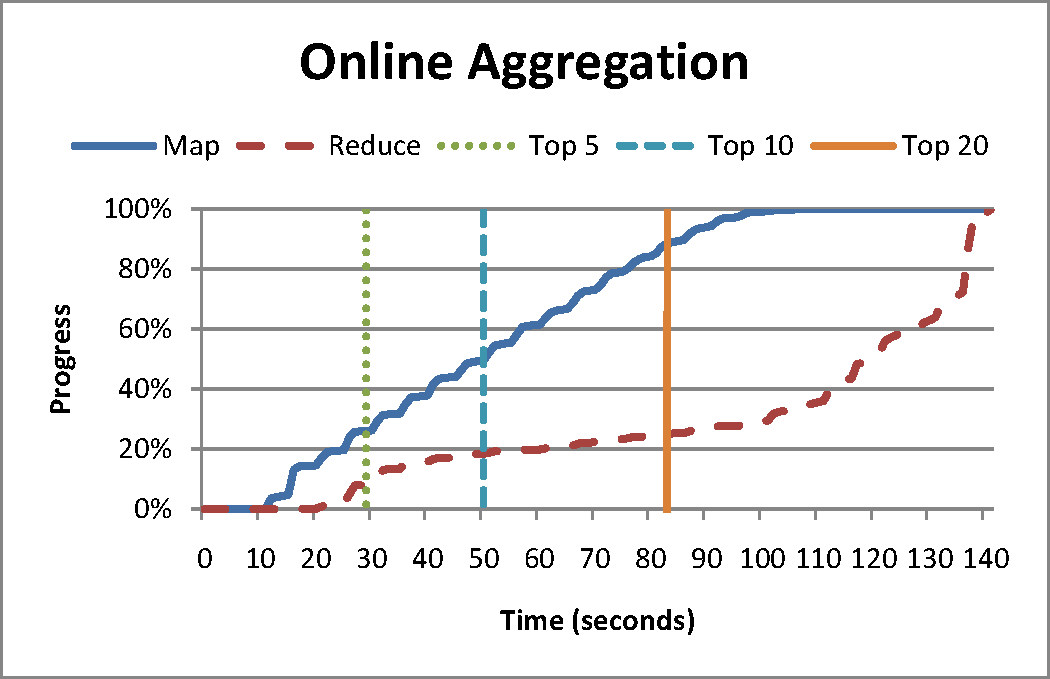
\includegraphics[width=0.95\linewidth]{eval/top100_online_wiki}
    \caption{Top-100 query over 5.5GB of Wikipedia article text. The vertical
      lines describe the increasing accuracy of the approximate answers produced
      by online aggregation.}
\label{fig:topkonlinewiki}
\vspace{-10pt}
\end{figure}

To evaluate the effectiveness of online aggregation, we performed two
experiments on Amazon EC2 using different data sets and query workloads. In our
first experiment, we wrote a ``Top-$K$'' query using two MapReduce jobs: the
first job counts the frequency of each word and the second job selects the $K$
most frequent words. We ran this workload on 5.5GB of Wikipedia article text
stored in HDFS, using a 128MB block size. We used a 60-node EC2 cluster; each
node was a ``high-CPU medium'' EC2 instance with 1.7GB of RAM and 2 virtual
cores. A virtual core is the equivalent of a 2007-era 2.5Ghz Intel Xeon
processor. A single EC2 node executed the Hadoop \JT\ and the HDFS \NN, while
the remaining nodes served as slaves for running the {\TT}s and HDFS {\DN}s.

% To evaluate inter-job dataflow with online aggregation we wrote a
% Top-$K$ query using two MapReduce jobs and executed it on 5.5GB of
% Wikipedia article text. The first job performs a wordcount on the
% words contained in each article.  A reducer from the first job will
% output a list of the Top-$K$ words observed in its partition. The key
% in this output is the word, and the value is the word count. Each map
% task in the subsequent job is assigned to an output from a single
% reduce task. The map function reverses the key-value order, and sends
% that result (sorted by count in descending order) to a single reduce
% task.  The single reduce task merges the sorted lists from each mapper
% and returns the first $K$ words.

% nrc: What does this experiment have to do with online aggregation?
% Figure~\ref{fig:topkwiki} reports the result of a Top-100 query over
% 5.5GB of Wikipedia article text. The left graph represents the
% blocking case as indicated by the idle period in the progress of the
% reduce tasks. The first map tasks finish around 100 seconds into the
% job, which is where the reduce tasks begin to make progress. The
% right graph shows a more balanced load. The reduce tasks
% being receiving mapper output almost immediately following the job
% execution, contributing to the early completion time of the job.

Figure~\ref{fig:topkonlinewiki} shows the results of inter-job online
aggregation for a Top-100 query. Our accuracy metric for this experiment is
post-hoc --- we note the time at which the Top-$K$ words in the snapshot are the
Top-$K$ words in the final result. Although the final result for this job did
not appear until nearly the end, we did observe the Top-5, 10, and 20 values at
the times indicated in the graph. The Wikipedia data set was biased toward these
Top-K words (e.g., ``the'', ``is'', etc.), which remained in their correct
position throughout the lifetime of the job.

\subsubsection{Approximation Metrics}

\begin{figure*}[ht]
  \centering
  \subfloat[][Relative approximation error over time]{\label{fig:approx-relative}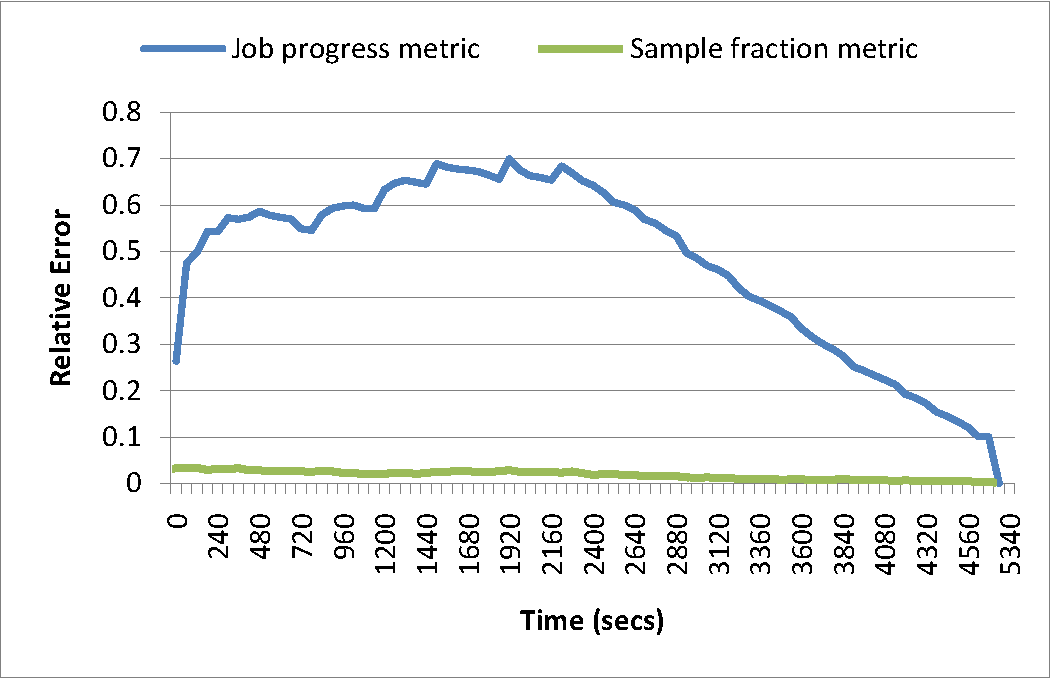
\includegraphics[width=0.48\linewidth]{eval/aprx-click-hour.pdf}}
  \hspace{4pt}
  \subfloat[][Example approximate answer]{\label{fig:approx-hour}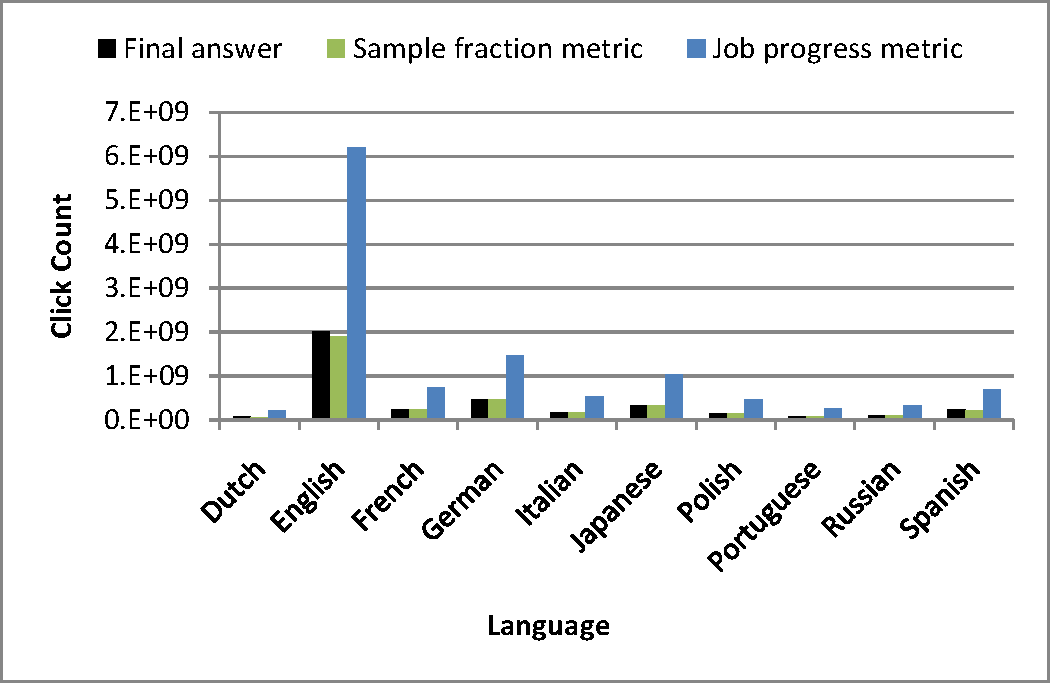
\includegraphics[width=0.48\linewidth]{eval/aprx-click-hour-actual.pdf}}
  \caption{Comparison of two approximation metrics. 
    Figure~\subref{fig:approx-relative} shows the relative error for
    each approximation metric over the runtime of the job, averaged over all
    groups. Figure~\subref{fig:approx-hour} compares an example approximate
    answer produced by each metric with the final answer, for each language and
    for a single hour.}
\label{fig:approx}
\end{figure*}

In our second experiment, we considered the effectiveness of the job progress
metric described in Section~\ref{sec:online-metric}. Unsurprisingly, this metric
can be inaccurate when it is used to estimate the accuracy of the approximate
answers produced by online aggregation. In this experiment, we compared the job
progress metric with a simple user-defined metric that leverages knowledge of
the query and data set. HOP allows such metrics, although developing such a
custom metric imposes more burden on the programmer than using the generic
progress-based metric.

We used a data set containing seven months of hourly page view statistics for
more than 2.5 million Wikipedia articles~\cite{wikistats}. This constituted
320GB of compressed data (1TB uncompressed), divided into 5066 compressed
files. We stored the data set on HDFS and assigned a single map task to each
file, which was decompressed before the map function was applied.

We wrote a MapReduce job to count the total number of page views for each
language and each hour of the day. In other words, our query grouped by language
and hour of day, and summed the number of page views that occurred in each
group. To enable more accurate approximate answers, we modified the map function
to include the fraction of a given hour that each record represents. The reduce
function summed these fractions for a given hour, which equated to one for all
records from a single map task. Since the total number of hours was known ahead
of time, we could use the result of this sum over all map outputs to determine
the total fraction of each hour that had been sampled. We call this user-defined
metric the ``sample fraction.''

To compute approximate answers, each intermediate result was scaled up using two
different metrics: the generic metric based on job progress and the sample
fraction described above. Figure~\ref{fig:approx-relative} reports the relative
error of the two metrics, averaged over all groups. Figure~\ref{fig:approx-hour}
shows an example approximate answer for a single hour using both metrics
(computed two minutes into the job runtime). This figure also contains the final
answer for comparison. Both results indicate that the sample fraction metric provides a
much more accurate approximate answer for this query than the progress-based
metric.

Job progress is clearly the wrong metric to use for approximating the final
answer of this query. The primary reason is that it is too coarse of a
metric. Each intermediate result was computed from some fraction of each
hour. However, the job progress assumes that this fraction is uniform across all
hours, when in fact we could have received much more of one hour and much less
of another. This assumption of uniformity in the job progress resulted in a
significant approximation error. By contrast, the sample fraction scales the
approximate answer for each group according to the actual fraction of data seen for
that group, yielding much more accurate approximations.
